\section{Geocoding}
We built a supervised disambiguation strategy for disambiguating mentions of location in text. The geolocation extraction performance of this new strategy is compared with the state-of-the-art geolocation model Mordecai (https://github.com/openeventdata/mordecai).  Both models are evaluated on English articles for the month of 2018-05 (we use only English for comparison, as Mordecai is only available for English). There are in total 1,743 events, of which 449 events have an approximate location, i.e, the location might not be directly mentioned in the text. We check if the event-location is among the disambiguated locations obtained from the location expressions in the text. The location expressions are obtained using a Named Entity Recognizer. The performance is shown in Figure.~\ref{fig:geoPerformance} .

\begin{figure}
    \centering
    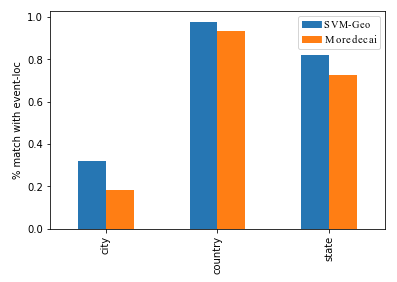
\includegraphics[width=0.6\textwidth]{figures/Geo_metrics.png}
    \caption{Performance comparison of the proposed geocoder vs state-of-the-art geo-coder Mordecai}
    \label{fig:geoPerformance}
\end{figure}

Our geocoding model works by first extracting all named entities namely Locations, Organizations and Person names, from text. We then query an elasticsearch database of Geonames for all possible expansions of a location entity mention. Once all possible expansions for a mention is obtained, we then decide which among the expansions is referred to in the text. This process is called Geo disambiguation. Most of the existing state-of-the-art methods like Kamalloo, et al. rely on hand-coded rules/hypotheses, e.g., location names mentioned consecutively share a common ancestor, names only refer to the most populous expansion, etc., for disambiguating location names.  Unlike these methods, we try to learn the rules automatically using machine learning. For each location expansion we built a feature set based on its frequency, the corresponding country and state frequency, distance to nearest mention of the corresponding country/state (both before and after), relative population of this expansion with respect to others etc. These features are then fed into a Random Forest classifier to decide which location a given named entity refers to. Since we do not use any features based on the words in the text, our method is language agnostic unlike other supervised geo disambiguation methods like Mordecai. Mordecai makes use of the words/context around a named entity mention to identify the country. We also query the organization names obtained to see if it mentions a country or state (for example, the entity “Indian Department of Treasury” gives hint about the country India). 
